
\section{Methodologies}
\label{sec6_2}

\subsection{Overview}

This section discusses the layout of the main methods used in processing and optimization of the meshes consisting the model surface.
The surface model of the vasculature used in this work was generated from the CTA information which was acquired from some real patient.
In order to put the model into the use of virtual interaction, the amount of information of the model have to be limited because of the constraints of the graphics hardware.
To limit the amount of information is equivalent to eliminate the total number of the polygonal elements that consist the model as much as possible, while preserving the original geometry of the vasculature. %

Some preprocessing steps illustrated in Fig. \ref{fig:DataFlow6} are necessary before the elimination of the polygons in the surface.
First of all, the validation of the connectivity among the vertices in the image-based model surface are performed to guarantee that the surface to be processed is complete as a whole and all the vertices are connected. %
Secondly, the smoothing step is introduced in order to depress the bulges and sunken areas in the connected surface.
Finally, the polygonal elements in the surface model are selected and part of them are deleted; the ``holes" left are patched and the geometry of the model is preserved as complete as possible. %

\subsection{Connectivity Validation}

Before any processing steps, one routine must be done to ensure that the surface model considered is well-shaped that no extra polygons exist in defining the same piece of surface.
This routine is designed to extract the polygons based on the geometric connectivity.
Concretely, it can extract the cells (i.e., polygons and/or triangles) that share the common points (i.e., vertices).

\subsection{Surface Smoothing}

In the field of computer graphics and imaging, the visualization of curves and surfaces (both will be referred to as \emph{shapes}) both in two- or three-dimensional space are common, especially for the volumetric data from medical field. %
The computation is in fact the proper approximation of the original shapes by the polygonal curves or polyhedral surfaces.
Typically, artifacts at certain level can be found in the resultant approximating shapes (see Fig. \ref{fig:Artifact}), and can be smoothed while maintaining the overall geometry (see Fig. \ref{fig:ArtifactRemoved}). %
In this work, one of our objectives is the smoothing or fairing of the model surface acquired by applying the iso-intensity extraction techniques on the raw medical images.
\begin{figure}[t]
\centering
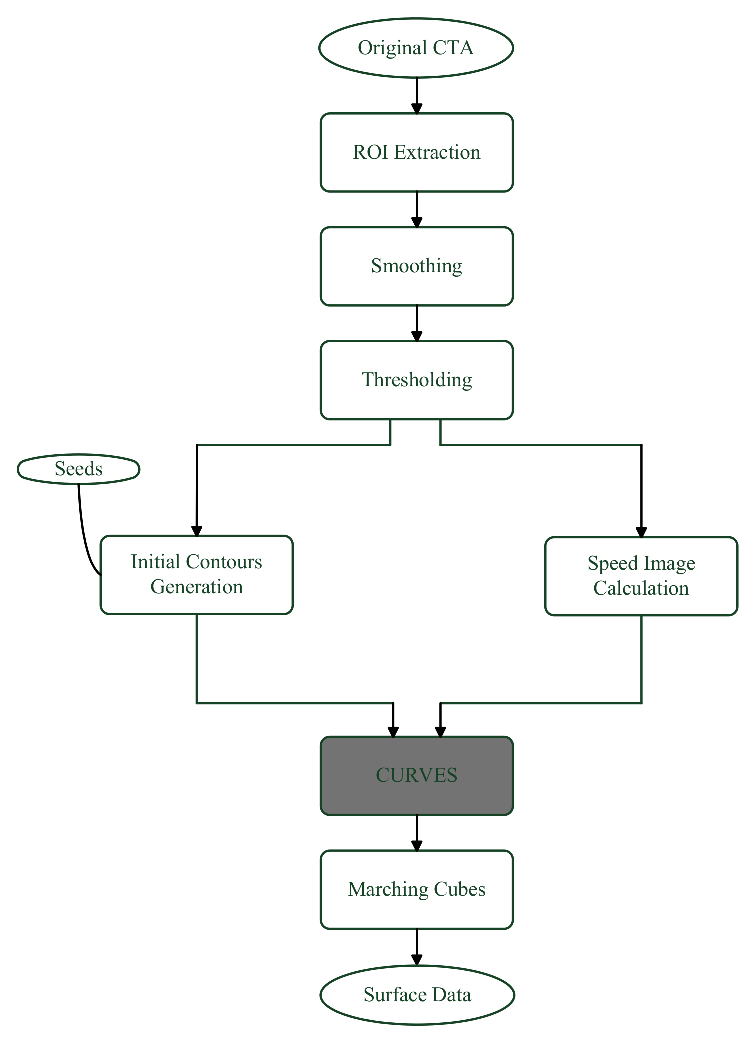
\includegraphics[width=3.2in]{figures/chap06/DataFlow.eps}
\caption{Overview of the work flow.}
\label{fig:DataFlow6}
\end{figure}
\begin{figure}[t]
\centering
\subfloat[]{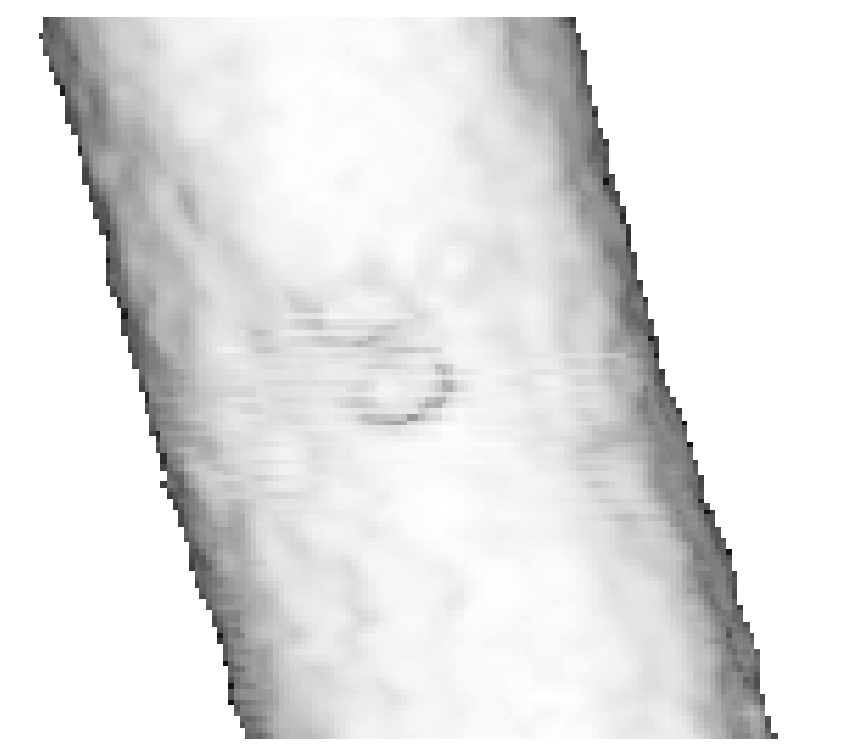
\includegraphics[height=1.0in]{figures/chap06/artifact.eps}%
\label{fig:Artifact}}
\hfil
\subfloat[]{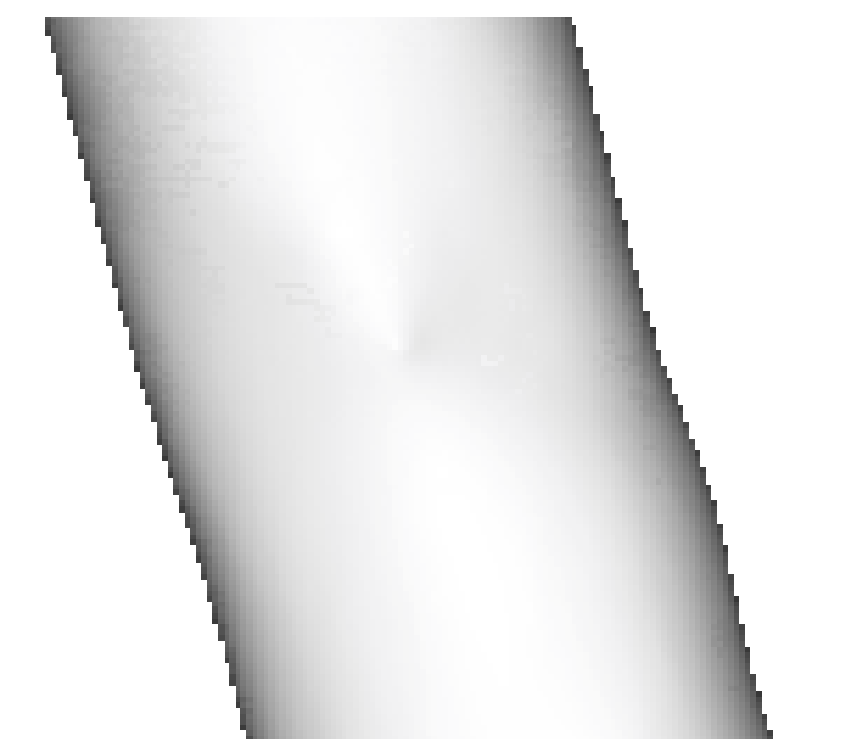
\includegraphics[height=1.0in]{figures/chap06/artifact_removed.eps}%
\label{fig:ArtifactRemoved}}
\caption{Smoothing the artifacts due to the approximation in visualization. (a) the artifacts (the horizontal ``steps" on the model surface of the vasculature); (b) the results after the smoothing process.}%
\label{fig:ArtifactComparison}
\end{figure}
A signal processing approach is employed to fulfill this task.
The approach is actually a linear low-pass filtering technique \cite{Taubin1995ICCV}, which is a low-level processing in the field of digital signal processing.
It can be applied to the smoothing process on the curves/surfaces of arbitrary dimension and complexities in geometry.
Moreover, no shrinkages will be introduced by the method during the computation.

The method is built upon the concepts of \emph{discrete graph signal} and its three-dimensional counterpart, \emph{discrete surface signal} \cite{Taubin1995SIG}.

By discrete graph signal, it means that some functions defined on the directed graph (\emph{digraph} for short).
Corresponding the polyhedral surfaces in consideration, the digraph $G$ can be marked as $G: \left\{ V_g, E\right\}$, where $V_g = \left\{ 1, \ldots, n \right\}$ is \emph{vertex set} including all the vertices in the graph, labeled from $1$ to $n$; and $E$ is the \emph{edge set} including the edges between any pair of vertices in the set $V_g$. %
The so-called discrete graph signal is a $n$-dimensional vector $x = \left[ x_1, \ldots, x_n \right]^T$, where the component $x_i, i = 1, \ldots, n$ denotes the signal intensity at the vertex $i \in V_g$. %

By discrete surface signal, it means that some functions defined on the polyhedral surfaces.
The polyhedral surfaces $S$ can be represented as $S: \left\{ V_s, F\right\}$, where $V_s = \left\{ 1, \ldots, n \right\}$ is \emph{vertex set} including all the vertices in the polyhedral surfaces, marked from $1$ to $n$; and $F$ is the set including the faces surrounded by the vertices in the set $V_s$ and the edges connecting them. %
The discrete surface signal is a $n$-dimensional vector $y = \left[ y_1, \ldots, y_n \right]^T$, where the component $y_j, j = 1, \ldots, n$ corresponds to the signal value at the vertex $j \in V_s$. %

For the smoothing of the planar polygonal curves, the classical Fourier analysis can be applied to decompose the original curves into orthogonal subspaces with distinct frequencies. %
After that, the components at high frequencies are removed as noises and the ones at low frequencies are left.
The idea can be extended to the case of the polyhedral surfaces with arbitrary topology.

For the discrete surface signal $y$, the weighted Laplacian operators for the vertices in $V_s$ are defined as
\begin{equation}
\label{eqn:Laplacian}
\Delta y_i = \sum_{j \in i^{\ast}} w_{ij} \left( y_j - y_i \right),
\end{equation}
where $w_{ij}$ is the positive weight for $y_j - y_i$, and for any $i$, the sum of its weights are always one, $\sum_{j \in i^{\ast}} w_{ij} = 1$.
The matrix form of (\ref{eqn:Laplacian}) is
\begin{equation}
\label{eqn:LaplacianMatrix}
\Delta y = - K y,
\end{equation}
where $K = I - W$, with $W$ the matrix of weights and $I$ an identity matrix.
Here we define $0 \leq \lambda_1 \leq \ldots \leq \lambda_n \leq 2$ as the real eigenvalues of $K$, and $e_1, \ldots, e_n$ the corresponding unit right eigenvectors.

At this point, the low-pass filtering can be presented as the multiplication of the matrix function $f(K)$ by the input signal $y$:
\begin{equation}
\label{eqn:LowPassEquivalent}
y' = f(K) y.
\end{equation}
For any polynomial transfer function, the output signal in (\ref{eqn:LowPassEquivalent}) can be rewritten as
\begin{equation}
\label{eqn:LowPassPolynomial}
y' = \sum_{i=1}^{n} \rho_i f(k_i) e_i,
\end{equation}
where $\rho_i$ are the coefficients of the linear combination of the unit right eigenvectors of the input signal $y$: $y = \sum_{i} \rho_i e_i$.
In order to realize a low pass filter, $f(k_i)$ is designed to satisfy two conditions: for $k_i \in [0,2]$, $f(k_i) \approx 1$ for low frequencies; $f(k_i) \approx 0$ for high frequencies. %

The low-pass filtering mechanism can be achieved by adjusting the weights in the following polynomial approximation \cite{Taubin1996}:
\begin{equation}
\label{eqn:Approximation}
f_{N}(k) = w_0 \frac{\theta}{\pi} T_0 (1 - k / 2) + w_n \sum_{n} \frac{2 \sin (n \theta)}{n \pi} T_n(1 - k / 2),
\end{equation}
where $\theta$ is the unique solution of $k = 2 (1 - \cos \theta)$ on $[0, \pi / 2]$, and $T_0(\cdot)$ and $T_n(\cdot)$ are the Chebyshev polynomials.
Here in this work, the weights in (\ref{eqn:Approximation}) is adjusted to form a Hamming window \cite{Taubin1996}, which can be represented as follows:
\begin{equation}
\label{eqn:HammingWindow}
w_n = 0.54 + 0.46 \cos (n \pi / (N + 1) ).
\end{equation}

After smoothing the surface, the normal vectors (\emph{normals} in short) are computed for each polygonal mesh.

\subsection{Polygons Decimation}
\label{subsec:decimation}

To eliminate the total number of polygons that consisting the model surface, an algorithm for the decimation of triangle meshes is employed in our approach \cite{Schroeder1992}.
The algorithm attempts to decimate certain rate of original meshes by firstly deleting the vertices whose coordinates are validated beforehand in the surface and then patching the holes left by creating a new triangulation at the location. %

All the vertices are labeled as simple, complex, and corners (see Fig. \ref{fig:FiveClasses}).
For simple vertices, two special cases are further specified as boundary vertices, and interior edge vertices.
\begin{figure}[t]
\centering
\subfloat[]{
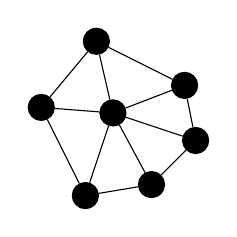
\begin{tikzpicture}[scale=.7,every node/.style={draw,shape=circle,fill=black,minimum size=1pt}]
% vertices
\path (0.5,1.5) node (p0) {}
(0,0) node (p1) {}
(1.2,0.2) node (p2) {}
(2,1) node (p3) {}
(1.8,2) node (p4) {}
(0.2,2.8) node (p5) {}
(-0.8,1.6) node (p6) {};
% edges
\draw (p0) -- (p1)
(p0) -- (p2)
(p0) -- (p3)
(p0) -- (p4)
(p0) -- (p5)
(p0) -- (p6)
(p1) -- (p2)
(p2) -- (p3)
(p3) -- (p4)
(p4) -- (p5)
(p5) -- (p6)
(p6) -- (p1);
\end{tikzpicture}
\label{fig:GeneralSimple}
}
\hfil
\subfloat[]{
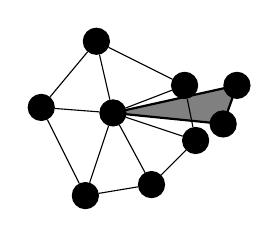
\begin{tikzpicture}[scale=.7,every node/.style={draw,shape=circle,fill=black,minimum size=1pt}]
\draw [fill=gray,thick] (0.5,1.5) -- (2.5,1.3) -- (2.75,2) -- (0.5,1.5);
% vertices
\path (0.5,1.5) node (p0) {}
(0,0) node (p1) {}
(1.2,0.2) node (p2) {}
(2,1) node (p3) {}
(1.8,2) node (p4) {}
(0.2,2.8) node (p5) {}
(-0.8,1.6) node (p6) {}
(2.5,1.3) node (p7) {}
(2.75,2) node (p8) {};
% edges
\draw (p0) -- (p1)
(p0) -- (p2)
(p0) -- (p3)
(p0) -- (p4)
(p0) -- (p5)
(p0) -- (p6)
(p1) -- (p2)
(p2) -- (p3)
(p3) -- (p4)
(p4) -- (p5)
(p5) -- (p6)
(p6) -- (p1);
\end{tikzpicture}
\label{fig:Complex}
}
\hfil
\subfloat[]{
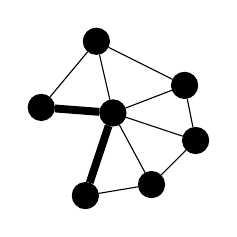
\begin{tikzpicture}[scale=.7,every node/.style={draw,shape=circle,fill=black,minimum size=1pt}]
% vertices
\path (0.5,1.5) node (p0) {}
(0,0) node (p1) {}
(1.2,0.2) node (p2) {}
(2,1) node (p3) {}
(1.8,2) node (p4) {}
(0.2,2.8) node (p5) {}
(-0.8,1.6) node (p6) {};
% edges
\draw (p0) -- (p1)
(p0) -- (p2)
(p0) -- (p3)
(p0) -- (p4)
(p0) -- (p5)
(p0) -- (p6)
(p1) -- (p2)
(p2) -- (p3)
(p3) -- (p4)
(p4) -- (p5)
(p5) -- (p6);
\draw [line width=.1cm] (p1) -- (p0) -- (p6);
\end{tikzpicture}
\label{fig:Boundary}
}
\hfil
\subfloat[]{
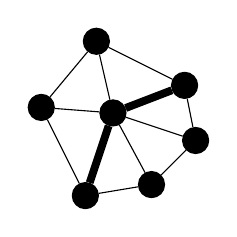
\begin{tikzpicture}[scale=.7,every node/.style={draw,shape=circle,fill=black,minimum size=1pt}]
% vertices
\path (0.5,1.5) node (p0) {}
(0,0) node (p1) {}
(1.2,0.2) node (p2) {}
(2,1) node (p3) {}
(1.8,2) node (p4) {}
(0.2,2.8) node (p5) {}
(-0.8,1.6) node (p6) {};
% edges
\draw (p0) -- (p1)
(p0) -- (p2)
(p0) -- (p3)
(p0) -- (p4)
(p0) -- (p5)
(p0) -- (p6)
(p1) -- (p2)
(p2) -- (p3)
(p3) -- (p4)
(p4) -- (p5)
(p5) -- (p6)
(p6) -- (p1);
\draw [line width=.1cm] (p1) -- (p0) -- (p4);
\end{tikzpicture}
\label{fig:InteriorEdge}
}
\hfil
\subfloat[]{
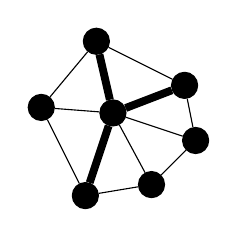
\begin{tikzpicture}[scale=.7,every node/.style={draw,shape=circle,fill=black,minimum size=1pt}]
% vertices
\path (0.5,1.5) node (p0) {}
(0,0) node (p1) {}
(1.2,0.2) node (p2) {}
(2,1) node (p3) {}
(1.8,2) node (p4) {}
(0.2,2.8) node (p5) {}
(-0.8,1.6) node (p6) {};
% edges
\draw (p0) -- (p1)
(p0) -- (p2)
(p0) -- (p3)
(p0) -- (p4)
(p0) -- (p5)
(p0) -- (p6)
(p1) -- (p2)
(p2) -- (p3)
(p3) -- (p4)
(p4) -- (p5)
(p5) -- (p6)
(p6) -- (p1);
\draw [line width=.1cm] (p1) -- (p0) -- (p4);
\draw [line width=.1cm] (p0) -- (p5);
\end{tikzpicture}
\label{fig:Corner}
}
\caption{Five classes of the vertex in the surface. (a) General simple case; (b) Complex case; (c) Boundary case; (d) Interior edge case; (e) Corner case. }%
\label{fig:FiveClasses}
\end{figure}
\begin{figure}[t]
\centering
\subfloat[]{
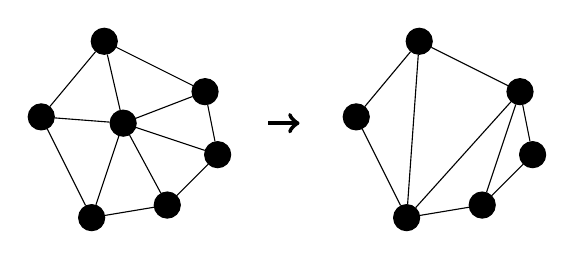
\begin{tikzpicture}[scale=.8,every node/.style={draw,shape=circle,fill=black,minimum size=3pt}]
% vertices
\path (0.5,1.5) node (p0) {}
(0,0) node (p1) {}
(1.2,0.2) node (p2) {}
(2,1) node (p3) {}
(1.8,2) node (p4) {}
(0.2,2.8) node (p5) {}
(-0.8,1.6) node (p6) {};
\path %(5.5,1.5) node (p7) {}
(5,0) node (p8) {}
(6.2,0.2) node (p9) {}
(7,1) node (p10) {}
(6.8,2) node (p11) {}
(5.2,2.8) node (p12) {}
(4.2,1.6) node (p13) {};
% edges
\draw (p0) -- (p1)
(p0) -- (p2)
(p0) -- (p3)
(p0) -- (p4)
(p0) -- (p5)
(p0) -- (p6)
(p1) -- (p2)
(p2) -- (p3)
(p3) -- (p4)
(p4) -- (p5)
(p5) -- (p6)
(p6) -- (p1);
\draw (p8) -- (p9)
(p9) -- (p10)
(p10) -- (p11)
(p11) -- (p12)
(p12) -- (p13)
(p13) -- (p8)
(p8) -- (p12)
(p8) -- (p11)
(p9) -- (p11);
% draw arrow
\draw [->,ultra thick] (2.8,1.5) -- (3.3,1.5);
\end{tikzpicture}
\label{fig:SimpleReduction}
}
\hfil
\subfloat[]{
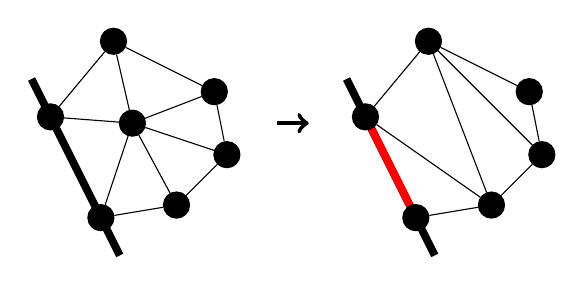
\begin{tikzpicture}[scale=.8,every node/.style={draw,shape=circle,fill=black,minimum size=3pt}]
% vertices
\path (0.5,1.5) node (p0) {}
(0,0) node (p1) {}
(1.2,0.2) node (p2) {}
(2,1) node (p3) {}
(1.8,2) node (p4) {}
(0.2,2.8) node (p5) {}
(-0.8,1.6) node (p6) {};
\path %(5.5,1.5) node (p7) {}
(5,0) node (p8) {}
(6.2,0.2) node (p9) {}
(7,1) node (p10) {}
(6.8,2) node (p11) {}
(5.2,2.8) node (p12) {}
(4.2,1.6) node (p13) {};
% edges
\draw (p0) -- (p1)
(p0) -- (p2)
(p0) -- (p3)
(p0) -- (p4)
(p0) -- (p5)
(p0) -- (p6)
(p1) -- (p2)
(p2) -- (p3)
(p3) -- (p4)
(p4) -- (p5)
(p5) -- (p6);
\draw [line width=0.1cm] (-1.1,2.2) -- (0.3,-0.6);
\draw (p8) -- (p9)
(p9) -- (p10)
(p10) -- (p11)
(p11) -- (p12)
(p12) -- (p13)
(p13) -- (p8)
(p9) -- (p13)
(p9) -- (p12)
(p10) -- (p12);
\draw [line width=0.1cm] (3.9,2.2) -- (5.3,-0.6);
\draw [line width=0.1cm,red] (p8) -- (p13);
% draw arrow
\draw [->,ultra thick] (2.8,1.5) -- (3.3,1.5);
\end{tikzpicture}
\label{fig:BoundaryReduction}
}
\caption{Reduction of polygons before and after eliminating the vertex. (a) General simple vertex case: number of polygons before reduction: $6$, number of polygons after reduction: $4$; (b) Boundary vertex case: number of polygons before reduction: $5$, number of polygons after reduction: $4$. Note that the edge in \emph{red} does not belong to the surface before the computation. }%
\label{fig:Reduction}
\end{figure}

To delete the unimportant vertices, some criteria must be designed and applied to validate the geometry of all potential targets among the model.
First of all, the complex vertices are definitely retained.
Then the rest are well checked to decide whether delete or not.
For the simple vertices that are not located on the boundary or the interior edge, the distance from them to the average plane is the unique principle -- if the distance is less than a certain value, it will be preserved; if not, it will be deleted. %
The vertices on the boundary or the interior edge are checked in the similar way -- if the distance is less than a certain value, it will be retained; otherwise, it will be kicked out. %
The vertices located at corners are usually preserved to maintain the approximation of the original geometry or left the ``noises" introduced in the modeling phase to be depressed by using appropriate method. %

Once upon the deletion of the vertex and its associated edges, one (in simple case) or two holes (in boundary or interior edge case) are left for patching thus maintaining the surface. In achieving the new patches for these holes, new triangulation at the location is created, which is done before the actual deletion mentioned before.

Comparing the number of triangles before and after this process, two triangles are reduced for the cases of general simple vertices, interior edge vertices, and some corner vertices; whilst one for the cases of vertices located at the boundaries (see Fig. \ref{fig:Reduction}). %
